\documentclass{beamer}
% \usetheme{Madrid}
\usepackage{tikz}
\usetikzlibrary{positioning}

% stuff for checkerboard
\usetikzlibrary{matrix.skeleton}
\tikzstyle{ball} = [circle, shading=ball, minimum size=1cm]
\newcommand{\bl}{\node [ball, ball color=black!80!white, draw=black!65!white, thin]{};}
\newcommand{\wh}{\node [ball, ball color=white] {};}



\begin{document}
    \title[NN and GA To Play Draughts] % (optional, only for long titles)
    {Playing Draughts using Neural Networks and Genetic Algorithms}
    \author[T. Nguyen] % (optional, for multiple authors)
    {Thien Nguyen}
    \institute[Durham] % (optional)
    {
    Department of Computer Science\\
    Durham University
    }
    \subject{Computer Science}

% Title Frame
\frame{\titlepage}


\begin{frame}

  \frametitle{Outline}
  %Content goes here
    %An outline: What are the elements of your talk?
    \begin{block}{Problem Description}
        % This is important information
     \end{block}
    \begin{block}{Motivation}
    % This is important information
    \end{block}
    \begin{block}{Related Work}
    % This is important information
    \end{block}
    \begin{block}{Approach}
    % This is important information
    \end{block}
    \begin{block}{Curent Progress}
    % This is important information
    \end{block}
    \begin{block}{Conclusion}
        % This is important information
    \end{block}
      
    %  \begin{alertblock}{This is an Alert block}
    %  This is an important alert
    %  \end{alertblock}
  
    %  \begin{exampleblock}{This is an Example block}
    %  This is an example 
    %  \end{exampleblock}
\end{frame}

% Plan for 8 minutes.

% A title slide: Project title, student name, course, date
%  An outline: What are the elements of your talk?
% A problem description, possibly both informal and formal
% Motivation: Why do you want to solve this problem? Previous work, and how it relates to what you are doing
% Your approach to solving the problem
% What you have accomplished so far (not relevant for marking!) Analysis: How will you judge the outcome of your work?
% A conclusion slide: What did or will you accomplish?
% What still needs to be done
\begin{frame}
  \frametitle{Problem Description}
  \framesubtitle{A problem in Computer Science}
    % More content goes here
    % Why is it important?
    % Currently (except for AlphaGo Zero) are really good at exploiting human games and definining "intuition" from there.
    Presently, competitive Draughts AI players are currently designed to play at a fixed ability. \\
    While it has produced very competitive and intelligent players, they require manual modifications in order to improve its performance. This is due to their dependency on pre-defined move databases, where optimal moves are pre-calculated, and recalled when necessary. \\
    By combining Neural Networks and Genetic Algorithms, this issue could possibly be solved by creating a player that can grow in ability over time, without the dependency on move-banks.


\end{frame}

\begin{frame}
    \frametitle{Motivation}
    \framesubtitle{Why have I chosen to tackle this?}
    % Why do you want to solve this problem? Previous work, and how it relates to what you are doing
    %More content goes here

    - Enjoyed the AI Search module \\
    - Want to learn about Machine Learning (unfortunately not an option this year) \\
    - I love board games! \\

    % Interested in neural networks, really enjoyed AI Search submodule. Inherent competitiveness against peers
    % Not necessarily interested in solving something new; also not expected for a bachelors degree.
\end{frame}

\begin{frame}
    \frametitle{Related Work}
    \framesubtitle{Similar works of art but no cigar}
    % Why do you want to solve this problem? Previous work, and how it relates to what you are doing
    \begin{block}{Samuel (59')}
        Uses Genetic Algorithms to improve coefficents of a set of heuristics to evaluate Draughts games.
    \end{block}
    %More content goes here
    \begin{block}{Blondie24 (97')}
        Uses an Evolutionary Algorithm and Neural Networks to evaluate Draughts games. (Quite similar!)
    \end{block}

     \begin{block}{Giraffe (15')}
        Uses contemporary machine learning techniques to train a Neural Network to evaluate Chess games.
     \end{block}
    % Interested in neural networks, really enjoyed AI Search submodule. Inherent competitiveness against peers
    % Not necessarily interested in solving something new; also not expected for a bachelors degree.
\end{frame}


\begin{frame}
    \frametitle{Current Approach}
    % Your approach to solving the problem
    \framesubtitle{How will I tackle this?}
    % Why do you want to solve this problem? Previous work, and how it relates to what you are doing
    %More content goes here
\end{frame}

% Neural Network Frame
\begin{frame}
    \frametitle{Neural Networks}
    \tikzset{%
    every neuron/.style={
    circle,
    draw,
    minimum size=1cm
    },
    neuron missing/.style={
    draw=none, 
    scale=4,
    text height=0.333cm,
    execute at begin node=\color{black}$\vdots$
    },
    }

    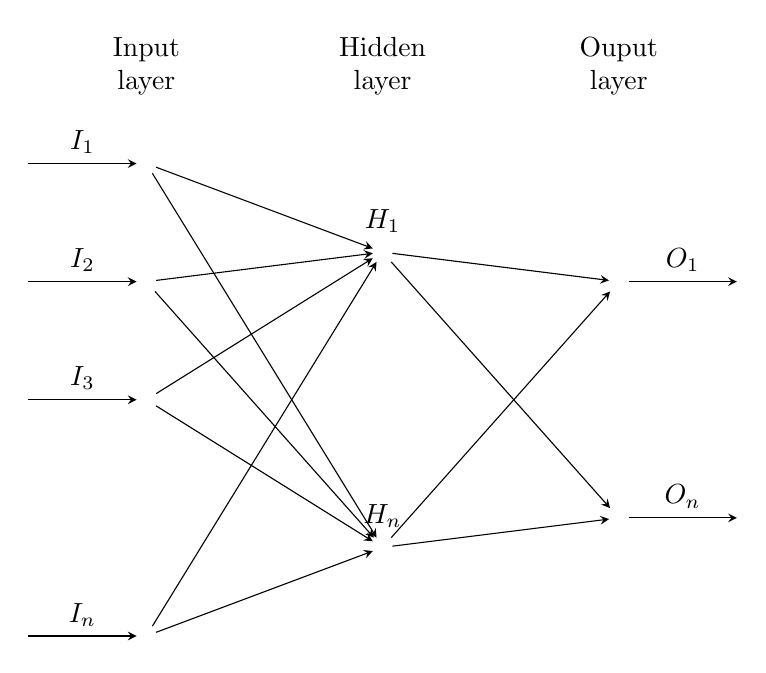
\begin{tikzpicture}[x=1.5cm, y=1.5cm, >=stealth]

    \foreach \m/\l [count=\y] in {1,2,3,missing,4}
    \node [every neuron/.try, neuron \m/.try] (input-\m) at (0,2.5-\y) {};

    \foreach \m [count=\y] in {1,missing,2}
    \node [every neuron/.try, neuron \m/.try ] (hidden-\m) at (2,2-\y*1.25) {};

    \foreach \m [count=\y] in {1,missing,2}
    \node [every neuron/.try, neuron \m/.try ] (output-\m) at (4,1.5-\y) {};

    \foreach \l [count=\i] in {1,2,3,n}
    \draw [<-] (input-\i) -- ++(-1,0)
    node [above, midway] {$I_\l$};

    \foreach \l [count=\i] in {1,n}
    \node [above] at (hidden-\i.north) {$H_\l$};

    \foreach \l [count=\i] in {1,n}
    \draw [->] (output-\i) -- ++(1,0)
    node [above, midway] {$O_\l$};

    \foreach \i in {1,...,4}
    \foreach \j in {1,...,2}
    \draw [->] (input-\i) -- (hidden-\j);

    \foreach \i in {1,...,2}
    \foreach \j in {1,...,2}
    \draw [->] (hidden-\i) -- (output-\j);

    \foreach \l [count=\x from 0] in {Input, Hidden, Ouput}
    \node [align=center, above] at (\x*2,2) {\l \\ layer};

    \end{tikzpicture}
\end{frame}


\begin{frame}
    \begin{wrapfigure}{l}{0.37 \textwidth}
        % \begin{center}
        \fontsize{8}{11}
        \vspace{-25pt}
        \centering
            \caption{The indexes of the 32 pieces of the input layer are the immediate values of the positions on the board. \label{boardarray}}
            \vspace{5pt}
            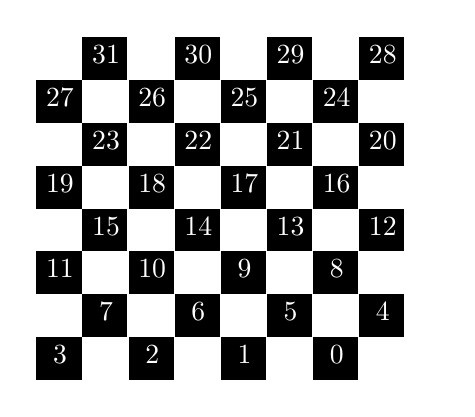
\begin{tikzpicture}
            \color{white}
            \matrix (m) [matrix of nodes, nodes in empty cells, label skeleton, nodes={minimum size = 0.4cm}] {
            & 31 &&30&&29&&28 \\
            27 &&26&&25&&24&&\\
            &23&&22&&21&&20\\   
                19&&18&&17&&16&&\\
            &15&&14&&13&&12\\
            11&&10&&9&&8&&\\
            &7&&6&&5&&4\\
            3&&2&&1&&0\\
            % \bl &     & \bl &     &     &     & \bl &     \\
            %     &     &     & \bl &     &     &     &     \\
            % \wh &     &     &     &     &     &     &     \\
            %     &     &     & \wh &     & \wh &     & \wh \\
            % \wh &     & \wh &     & \wh &     & \wh &     \\
            %     & \wh &     & \wh &     & \wh &     & \wh \\
            };
            \foreach \row in {1, ..., 8} {
            \foreach \col in {1, ..., 8} {
                \pgfmathparse{Mod(\row + \col, 2) ? "black" : "white"}
                \colorlet{squarebg}{\pgfmathresult}
                \fitandstyle[background]{(m-cell-\row-\col)}{fill = squarebg}
            }
            }
            \end{tikzpicture}
        % \end{center}
      
    \end{wrapfigure}
\end{frame}

% ----------------------------

\begin{frame}
    \frametitle{Current Progress}
    % Your approach to solving the problem
    % How will I Judge the outcome of the work?
    \framesubtitle{What have I done already?}

    - I've created a relatively ok AI bot. \\
    - It plays relatively well! \\

\end{frame}

\begin{frame}
    \frametitle{Remaining Work}
    \framesubtitle{What do I still need to do?}
    % What did or will you accomplish?
    % What still needs to be done
    % \framesubtitle{A bit more information about this}
\end{frame}

\begin{frame}
    \frametitle{Conclusion}
    \framesubtitle{What will I accomplish?}
    % What did or will you accomplish?
    % What still needs to be done
    % \framesubtitle{A bit more information about this}
\end{frame}

\begin{frname}
    \frametitle{References}
    \framesubtitle{Nanos gigantum humeris insidentes}
    % What did or will you accomplish?
    % What still needs to be done
    % \framesubtitle{A bit more information about this}
\end{frame}


% etc
\end{document}